% =========================================================
\subsubsection{Balls in Metric Spaces}
\label{sec:balls-metric-spaces}
% =========================================================

% ---- Toolkit ----
\begin{tcolorbox}[colback=gray!6, colframe=gray!40, arc=2pt,
  left=6pt, right=6pt, top=4pt, bottom=4pt,
  title={\small\textbf{Balls in Metric Spaces --- Quick Reference}},
  fonttitle=\small\bfseries]
\small
\begin{tabular}{l l l l}
\toprule
\textbf{Label} & \textbf{Statement} & \textbf{Proof method} & \textbf{Detail} \\
\midrule
D\ref{def:open-ball}
  & $B_r(x) := \{\,y\in X : d(x,y) < r\,\}$
  & Definition
  & \hyperref[def:open-ball]{$\downarrow$} \\
D\ref{def:closed-ball}
  & $\overline{B}_r(x) := \{\,y\in X : d(x,y) \le r\,\}$
  & Definition
  & \hyperref[def:closed-ball]{$\downarrow$} \\
D\ref{def:open-closed-set}
  & Open: $\forall x\in S,\;\exists r>0,\;B_r(x)\subseteq S$
  & Definition
  & \hyperref[def:open-closed-set]{$\downarrow$} \\
P\ref{prop:balls-open-closed}
  & $B_r(x)$ is open;\; $\overline{B}_r(x)$ is closed
  & Triangle inequality
  & \hyperref[prop:balls-open-closed]{$\downarrow$} \\
\bottomrule
\end{tabular}
\end{tcolorbox}

% ---- Open Ball ----
\begin{tcolorbox}[colback=propbox, colframe=propborder, arc=2pt,
  left=6pt, right=6pt, top=4pt, bottom=4pt,
  title={\small\textbf{Definition (Open Ball)}},
  fonttitle=\small\bfseries]
\begin{definition}[Open Ball]
\label{def:open-ball}
Let $(X,d)$ be a metric space.
For $x \in X$ and $r > 0$, the \emph{open ball} centred at $x$ with radius $r$ is
\[
B_r(x)
:=
\{\, y \in X : d(x,y) < r \,\}.
\]
\end{definition}
\end{tcolorbox}

\begin{remark*}[Fully quantified form]
$\forall (X,d)\ \text{metric space},\;
 \forall x \in X,\;
 \forall r \in \mathbb{R}^{+},\quad
 B_r(x) := \{\, y \in X : d(x,y) < r \,\}.$
\end{remark*}

\begin{tikzpicture}[
  dot/.style={circle,fill,inner sep=1.9pt},
  >=Stealth,
  lbl/.style={font=\small},
  slbl/.style={font=\scriptsize},
]

% ═══ Geometry (world coords) ══════════════════════════════════
%   x   = (-1.4, 0)   — centre of B_r(x)
%   x0  = ( 0.6, 0.7) — interior point; |x0-x|=(2.0,0.7) ≈ 2.12
%   x1  = (-0.3, 1.4) — inside B_eps(x0); |x1-x0|=(0.9,0.7) ≈ 1.14 ≈ eps
%   R   = 3.8          — outer radius   (|x0-x|+eps ≈ 2.12+1.15 = 3.27 < 3.8)
%   eps = 1.15         — inner radius
%
%   x1 sits clearly to the UPPER-LEFT of x0, giving label space.
%   The gap arrow goes UPPER-RIGHT (toward the outer boundary along x→x0 ray).

\coordinate (x)  at (-1.4,  0.0);
\coordinate (x0) at ( 0.6,  0.7);
\coordinate (x1) at (-0.3,  1.6);

\def\R{3.8}
\def\eps{1.15}

% ─── Filled regions ───────────────────────────────────────────
\fill[blue!7]    (x)  circle (\R);
\fill[orange!16] (x0) circle (\eps);

% ─── Boundaries ───────────────────────────────────────────────
\draw[blue!55!black,   line width=1.4pt, dashed] (x)  circle (\R);
\draw[orange!60!black, line width=1.2pt]         (x0) circle (\eps);

% ─── Points ───────────────────────────────────────────────────
\node[dot, fill=blue!70!black]   at (x)  {};
\node[dot, fill=orange!75!black] at (x0) {};
\node[dot, fill=red!65!black]    at (x1) {};

% ─── Point labels ─────────────────────────────────────────────
\node[lbl, anchor=north]      at ($(x)  + (0,-0.14)$)   {$x$};
\node[lbl, anchor=north west] at ($(x0) + (0.10,-0.12)$) {$x_0$};
\node[lbl, anchor=south]      at ($(x1) + (0, 0.12)$)   {$x_1$};

% ─── x → x0  blue solid ────────────────────────────────────
\draw[blue!65!black, line width=1.0pt] (x) -- (x0);
\node[slbl, text=blue!65!black, anchor=north]
  at ($(x)!0.5!(x0) + (0,-0.10)$) {$d(x,x_0)$};

% ─── x0 → x1  orange solid ─────────────────────────────────
\draw[orange!75!black, line width=1.0pt] (x0) -- (x1);
\node[slbl, text=orange!75!black, anchor=east]
  at ($(x0)!0.5!(x1) + (-0.12, 0)$) {$d(x_0,x_1)$};

% ─── x → x1  red dashed ────────────────────────────────────
\draw[red!55!black, line width=0.9pt, dashed] (x) -- (x1);
\node[slbl, text=red!50!black, anchor=east]
  at ($(x)!0.45!(x1) + (-0.10, 0)$) {$d(x,x_1)$};

% ─── Radius r  (rightward, below x) ─────────────────────────
\draw[blue!50!black, line width=0.8pt, <->]
  ($(x)+(0,-0.70)$) -- ++({\R},0)
  node[midway, slbl, below, yshift=-3pt, text=blue!55!black] {$r$};

% ─── Boundary point along x→x0 direction ─────────────────────
% x0 relative to x = (0.6-(-1.4), 0.7-0.0) = (2.0, 0.7)
\pgfmathsetmacro{\relx}{2.0}
\pgfmathsetmacro{\rely}{0.7}
\pgfmathsetmacro{\dxo}{sqrt(\relx*\relx+\rely*\rely)}
\pgfmathsetmacro{\ux}{\relx/\dxo}
\pgfmathsetmacro{\uy}{\rely/\dxo}
\pgfmathsetmacro{\bwx}{-1.4 + \ux*\R}
\pgfmathsetmacro{\bwy}{ 0.0 + \uy*\R}
\node[dot, fill=blue!40!black, inner sep=1.0pt] at (\bwx,\bwy) {};

% ─── Gap arrow x0 → boundary, label above ────────────────────
\draw[gray!55, line width=0.78pt, <->] (x0) -- (\bwx,\bwy);
% midpoint of gap segment, shift label above the line
\node[slbl, text=gray!55!black, anchor=south west]
  at ($(x0)!0.46!(\bwx,\bwy) + (0.0, 0.18)$) {$r - d(x,x_0)$};

% ─── ε arrow downward from x0 ────────────────────────────────
\draw[orange!60!black, line width=0.8pt, <->]
  (x0) -- ++(0,-\eps)
  node[midway, slbl, right, xshift=4pt, text=orange!70!black] {$\varepsilon$};

% ─── Ball name labels ─────────────────────────────────────────
% B_r(x): lower-left interior where there is clear space
\node[lbl, text=blue!60!black, font=\small\itshape]
  at ($(x) + (-2.4,-1.8)$) {$B_r(x)$};

% B_eps(x0): lower-right of inner ball, outside it
\node[lbl, text=orange!65!black, font=\small\itshape]
  at ($(x0) + (1.05,-0.65)$) {$B_\varepsilon(x_0)$};

% ─── Choice annotation ────────────────────────────────────────
\node[slbl, text=gray!50!black, font=\scriptsize\itshape, anchor=north west]
  at ($(x)+(-2.4,-2.25)$)
  {choose $\varepsilon$ with $0 < \varepsilon < r - d(x,x_0)$};

% ─── Callout box ──────────────────────────────────────────────
\node[
  draw=gray!40, fill=white, rounded corners=4pt,
  font=\scriptsize, text width=7.0cm,
  align=left, inner sep=8pt, anchor=north west
] at ($(x)+(-2.4,-2.65)$) {
  \textbf{Triangle inequality:}\\[5pt]
  $d(x,x_1) \;\leq\; d(x,x_0) + d(x_0,x_1)$\\[3pt]
  $\phantom{d(x,x_1)}\;< (r-\varepsilon)+\varepsilon$\\[3pt]
  $\phantom{d(x,x_1)}\;= r$\\[5pt]
  $\therefore$ $x_1\in B_r(x)$.
  Since $x_1\in B_\varepsilon(x_0)$ was arbitrary,
  $B_\varepsilon(x_0)\subseteq B_r(x)$.
};

\end{tikzpicture}

\begin{remark*}[Intuition]
The open ball is the metric-space generalisation of an open interval in $\mathbb{R}$.
In $(\mathbb{R}, |\cdot|)$ it recovers the interval $(x-r, x+r)$.
In $(\mathbb{R}^2, \|\cdot\|_2)$ it is the open disc of radius $r$.
The strict inequality $d(x,y) < r$ means the boundary circle is excluded.
\end{remark*}
\begin{remark*}
Every point of an open ball has positive distance from the boundary of the ball.
This allows a smaller ball to be placed around any interior point.
\end{remark*}

% ---- Closed Ball ----
\begin{tcolorbox}[colback=propbox, colframe=propborder, arc=2pt,
  left=6pt, right=6pt, top=4pt, bottom=4pt,
  title={\small\textbf{Definition (Closed Ball)}},
  fonttitle=\small\bfseries]
\begin{definition}[Closed Ball]
\label{def:closed-ball}
Let $(X,d)$ be a metric space.
For $x \in X$ and $r > 0$, the \emph{closed ball} centred at $x$ with radius $r$ is
\[
\overline{B}_r(x)
:=
\{\, y \in X : d(x,y) \le r \,\}.
\]
\end{definition}
\end{tcolorbox}

\begin{remark*}[Fully quantified form]
$\forall (X,d)\ \text{metric space},\;
 \forall x \in X,\;
 \forall r \in \mathbb{R}^{+},\quad
 \overline{B}_r(x) := \{\, y \in X : d(x,y) \le r \,\}.$
\end{remark*}


\begin{tikzpicture}

\coordinate (x)  at (0,   0);
\coordinate (x0) at (6.4, 2.7);   % raised ~1 inch above x

\def\R{2.2}      % interpreted as cm when used in circle()
\def\EPS{0.80}   % interpreted as cm when used in circle()

% rpt: boundary of closed ball toward x0 (DISTANCE \R cm from x toward x0)
\coordinate (rpt)      at ($(x)!\R cm!(x0)$);

% nearEdge: boundary of eps-ball toward x (DISTANCE \EPS cm from x0 toward x)
\coordinate (nearEdge) at ($(x0)!\EPS cm!(x)$);

% x1: inside eps-ball
\coordinate (x1)       at ($(x0)+(-0.30, 0.55)$);

%--- filled regions ---
\fill[blue!10]   (x)  circle (\R);
\fill[orange!20] (x0) circle (\EPS);

%--- boundaries ---
\draw[blue!65!black, very thick]      (x)  circle (\R);
\draw[orange!60!black, thick, dashed] (x0) circle (\EPS);

%--- triangle lines: x->x1, x1->x0, x->x0 (faint) ---
\draw[gray!50, thin] (x)  -- (x0);   % d(x,x0) reference
\draw[gray!50, thin] (x)  -- (x1);   % d(x,x1)
\draw[gray!50, thin] (x1) -- (x0);   % d(x1,x0) = d(x0,x1)

%--- r segment with ticks ---
\draw[blue!60!black, thick] (x) -- (rpt);

% perpendicular ticks (rotate 90 around the segment direction)
\pgfmathanglebetweenpoints{\pgfpointanchor{x}{center}}{\pgfpointanchor{x0}{center}}
\let\ang\pgfmathresult

\draw[blue!60!black, thick]
    ($(x)+(\ang+90:0.13)$) -- ($(x)+(\ang-90:0.13)$);
\draw[blue!60!black, thick]
    ($(rpt)+(\ang+90:0.13)$) -- ($(rpt)+(\ang-90:0.13)$);

\node[blue!60!black, font=\small, below=5pt] at ($0.5*(x)+0.5*(rpt)$) {$r$};

%--- gap bracket along the x-x0 line, offset to the side ---
% midpoint of gap
\coordinate (gapMid) at ($0.5*(rpt)+0.5*(nearEdge)$);

% offset perpendicular to x-x0 line (toward bottom-right)
\coordinate (gapMidOff)   at ($(gapMid)+(\ang-90:0.45)$);
\coordinate (rptOff)      at ($(rpt)+(\ang-90:0.45)$);
\coordinate (nearEdgeOff) at ($(nearEdge)+(\ang-90:0.45)$);

\draw[red!60!black, thin, dotted] (rpt)      -- (rptOff);
\draw[red!60!black, thin, dotted] (nearEdge) -- (nearEdgeOff);

\draw[red!60!black, thick, {Bar[width=6pt]}-{Bar[width=6pt]}]
    (rptOff) -- (nearEdgeOff);

\node[red!60!black, font=\small, below=4pt] at (gapMidOff)
    {$d(x,x_0){-}r{-}\varepsilon > 0$};

%--- d(x,x0) label above the midpoint of whole segment ---
\node[gray!55, font=\footnotesize, above=3pt] at ($0.5*(x)+0.5*(x0)$)
    {$d(x,x_0)$};

%--- epsilon line inside eps-ball ---
\draw[orange!60!black, thick] (x0) -- (x1);
\node[orange!60!black, font=\small, left=2pt] at ($0.5*(x0)+0.5*(x1)$)
    {$\varepsilon$};

%--- points ---
\filldraw[black]         (x)   circle (2.4pt) node[below left,  font=\small] {$x$};
\filldraw[black]         (x0)  circle (2.4pt) node[right=4pt,   font=\small] {$x_0$};
\filldraw[black]         (x1)  circle (2.0pt) node[above left,  font=\small] {$x_1$};
\filldraw[blue!65!black] (rpt) circle (1.8pt);

%--- ball labels ---
\node[blue!65!black,   font=\small] at ($(x) +(135:\R *0.58)$)  {$\overline{B}_r(x)$};
\node[orange!60!black, font=\small] at ($(x0)+(50:\EPS*1.85)$)  {$B_\varepsilon(x_0)$};

%--- inequality box ---
\node[draw=gray!40, fill=gray!5, rounded corners=5pt,
      font=\footnotesize, align=left, inner sep=8pt]
  at (2.2, -2.6) {%
    $d(x_0,x_1) < \varepsilon$\\[3pt]
    $d(x,x_0) \le d(x,x_1)+d(x_1,x_0)$\\[3pt]
    $\varepsilon + r < d(x,x_0) \le d(x,x_1)+\varepsilon$\\[3pt]
    $\therefore\ r < d(x,x_1)
       \;\Rightarrow\; x_1 \notin \overline{B}_r(x)$};

\end{tikzpicture}

\begin{remark*}[Common error]
The closure of the open ball $\overline{B_r(x)}$ need not equal the closed
ball $\overline{B}_r(x)$ in a general metric space.
In $\mathbb{R}^n$ with the standard metric they agree, but in a discrete metric
space $B_r(x) = \{x\}$ for $r \le 1$ and $\overline{B_r(x)} = \{x\}$ while
$\overline{B}_r(x) = X$ for $r = 1$.
The notation is therefore intentionally distinct.
\end{remark*}

% =========================================================
% TikZ diagram: Open ball vs. Closed ball (side-by-side)
% Place after the Closed Ball definition box.
% Requires: \usepackage{tikz}  \usetikzlibrary{calc}
%           \usepackage{caption}   (for \captionof)
% =========================================================

\begin{center}
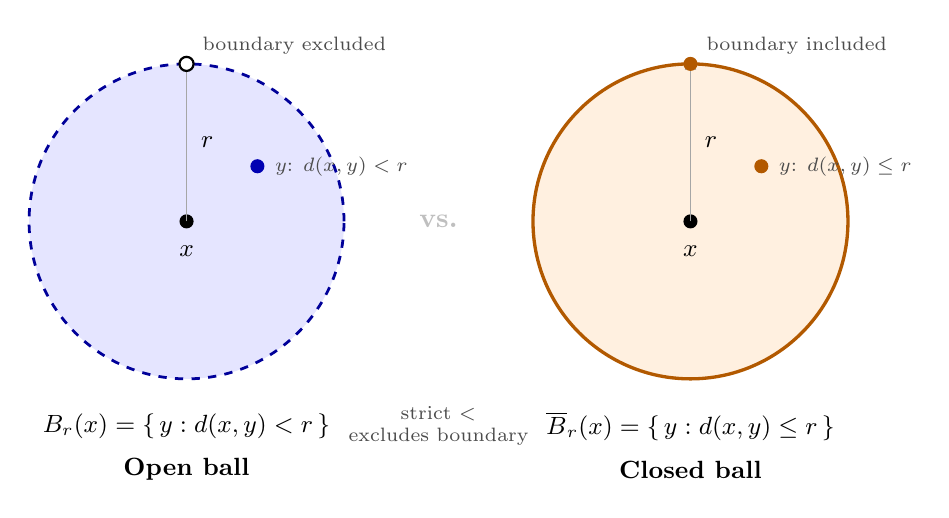
\begin{tikzpicture}[
  dot/.style     = {circle, fill, inner sep=1.8pt},
  opendot/.style = {circle, draw, fill=white, inner sep=1.8pt, line width=0.8pt},
  lbl/.style     = {font=\small},
  sublbl/.style  = {font=\scriptsize, text=gray!60!black}
]

% ---- LEFT PANEL: Open ball ----
\begin{scope}[shift={(-3.2,0)}]
  \fill[blue!10] (0,0) circle (2cm);
  \draw[blue!60!black, dashed, line width=1.0pt] (0,0) circle (2cm);
  \node[dot, fill=black] at (0,0) {};
  \node[lbl, anchor=north] at (0,-0.18) {$x$};
  \draw[->, gray!70, line width=0.6pt] (0,0) -- (0,2);
  \node[lbl, anchor=west] at (0.06, 1.0) {$r$};
  \node[opendot] at (0,2) {};
  \node[sublbl, anchor=south west] at (0.08, 2.0) {boundary excluded};
  \node[dot, fill=blue!70!black] at (0.9, 0.7) {};
  \node[sublbl, anchor=west] at (1.0, 0.7) {$y$: $d(x,y) < r$};
  \node[lbl] at (0, -2.6) {$B_r(x) = \{\,y : d(x,y) < r\,\}$};
  \node[lbl, font=\small\bfseries] at (0, -3.15) {Open ball};
\end{scope}

% ---- VS divider ----
\node[font=\normalsize\bfseries, text=gray!50] at (0, 0) {vs.};
\node[sublbl, align=center] at (0, -2.6)
  {strict $<$\\excludes boundary};

% ---- RIGHT PANEL: Closed ball ----
\begin{scope}[shift={(3.2,0)}]
  \fill[orange!12] (0,0) circle (2cm);
  \draw[orange!70!black, solid, line width=1.2pt] (0,0) circle (2cm);
  \node[dot, fill=black] at (0,0) {};
  \node[lbl, anchor=north] at (0,-0.18) {$x$};
  \draw[->, gray!70, line width=0.6pt] (0,0) -- (0,2);
  \node[lbl, anchor=west] at (0.06, 1.0) {$r$};
  \node[dot, fill=orange!70!black] at (0,2) {};
  \node[sublbl, anchor=south west] at (0.08, 2.0) {boundary included};
  \node[dot, fill=orange!70!black] at (0.9, 0.7) {};
  \node[sublbl, anchor=west] at (1.0, 0.7) {$y$: $d(x,y) \le r$};
  \node[lbl] at (0, -2.6)
    {$\overline{B}_r(x) = \{\,y : d(x,y) \le r\,\}$};
  \node[lbl, font=\small\bfseries] at (0, -3.15) {Closed ball};
\end{scope}

\end{tikzpicture}
\captionof{figure}{Open ball $B_r(x)$ (left) versus closed ball $\overline{B}_r(x)$
(right) in a metric space $(X,d)$.
The dashed boundary of $B_r(x)$ indicates that boundary points satisfying
$d(x,y)=r$ are \emph{excluded} (strict inequality); the solid boundary of
$\overline{B}_r(x)$ indicates they are \emph{included} ($\le$).}
\label{fig:open-closed-balls}
\end{center}

\begin{remark*}[Interior points of a ball]
Every point inside a ball that is not on the boundary admits a smaller
open ball around it.

Let $(X,d)$ be a metric space and let $y \in B_r(x)$, so that
\[
d(x,y) < r.
\]
Define
\[
\varepsilon := r - d(x,y) > 0.
\]
Then
\[
B_{\varepsilon}(y) \subseteq B_r(x).
\]

Geometrically, the quantity $r - d(x,y)$ represents the remaining
distance from $y$ to the boundary of the ball $B_r(x)$.
Thus a smaller open ball centered at $y$ fits entirely inside $B_r(x)$.
\end{remark*}

\begin{remark}[Intervals generalise to balls]
In $(\mathbb{R},|\cdot|)$, open balls coincide with open intervals and
closed balls coincide with closed intervals:

\[
B_r(x) = (x-r,x+r), \qquad \overline{B}_r(x) = [x-r,x+r].
\]

Thus open and closed intervals on the real line generalise naturally
to open and closed balls in metric spaces.
\end{remark}



% ---- Open Set and Closed Set ----
\begin{tcolorbox}[colback=propbox, colframe=propborder, arc=2pt,
  left=6pt, right=6pt, top=4pt, bottom=4pt,
  title={\small\textbf{Definition (Open Set, Closed Set)}},
  fonttitle=\small\bfseries]
\begin{definition}[Open Set, Closed Set]
\label{def:open-closed-set}
Let $(X, d)$ be a metric space and $S \subseteq X$.
\begin{itemize}
  \item $S$ is \emph{open} (in $X$) if for every $x \in S$ there exists
        $r > 0$ such that $B_r(x) \subseteq S$.
  \item $S$ is \emph{closed} (in $X$) if its complement $X \setminus S$
        is open.
\end{itemize}
\end{definition}
\end{tcolorbox}

\begin{remark*}[Fully quantified form]
\begin{align*}
S\ \text{open}
  &\iff \forall x \in S,\;
         \exists r \in \mathbb{R}^{+},\;
         B_r(x) \subseteq S. \\
S\ \text{closed}
  &\iff X \setminus S\ \text{is open} \\
  &\iff \forall x \in X \setminus S,\;
         \exists r \in \mathbb{R}^{+},\;
         B_r(x) \subseteq X \setminus S.
\end{align*}
\end{remark*}

\begin{remark*}[Common error]
Open and closed are \emph{not} opposites.
A set can be both open and closed (e.g.\ $\emptyset$ and $X$ itself),
or neither (e.g.\ the half-open interval $[0,1)$ in $\mathbb{R}$).
\end{remark*}

% =========================================================
% TikZ diagram: Open set definition
% Place after the Open Set / Closed Set definition box.
% Requires: \usepackage{tikz}  \usetikzlibrary{calc}
%           \usepackage{caption}   (for \captionof)
% =========================================================

\begin{center}
\begin{tikzpicture}[
  dot/.style     = {circle, fill, inner sep=1.8pt},
  lbl/.style     = {font=\small},
  sublbl/.style  = {font=\scriptsize, text=gray!55!black}
]

% --- Open set S ---
\fill[blue!10]
  (0, -0.3)
  .. controls ( 1.4,  0.2) and ( 2.2,  1.4) .. ( 1.8,  2.8)
  .. controls ( 1.2,  4.0) and (-0.6,  4.4) .. (-1.8,  3.6)
  .. controls (-3.2,  2.8) and (-3.4,  1.0) .. (-2.4,  0.0)
  .. controls (-1.6, -0.8) and (-0.6, -0.6) .. ( 0,   -0.3)
  -- cycle;

\draw[blue!55!black, dashed, line width=0.9pt]
  (0, -0.3)
  .. controls ( 1.4,  0.2) and ( 2.2,  1.4) .. ( 1.8,  2.8)
  .. controls ( 1.2,  4.0) and (-0.6,  4.4) .. (-1.8,  3.6)
  .. controls (-3.2,  2.8) and (-3.4,  1.0) .. (-2.4,  0.0)
  .. controls (-1.6, -0.8) and (-0.6, -0.6) .. ( 0,   -0.3)
  -- cycle;

\node[lbl, text=blue!60!black, font=\small\itshape] at (-1.5, 0.6) {$S$};
\node[lbl, font=\small\itshape] at (-3.8, 4.2) {$X$};

% --- Interior point x: ball fits ---
\coordinate (x1) at (-0.8, 2.2);
\draw[blue!70!black, dashed, line width=0.7pt] (x1) circle (0.85cm);
\draw[gray!60, line width=0.6pt, ->] (x1) -- ++(0.85, 0);
\node[sublbl, anchor=south] at ($(x1)+(0.42, 0.0)$) {$r$};
\node[dot, fill=blue!70!black] at (x1) {};
\node[lbl, anchor=south east] at ($(x1)+(-0.08, 0.10)$) {$x$};
\node[sublbl, anchor=south, align=center] at ($(x1)+(0, 0.92)$)
  {$B_r(x)\subseteq S$ \quad \textit{fits inside}};

% --- Near-boundary point z: ball leaks ---
\coordinate (z) at (1.35, 1.7);
\draw[red!60!black, dashed, line width=0.7pt] (z) circle (0.52cm);
\node[dot, fill=red!70!black] at (z) {};
\node[lbl, anchor=north west] at ($(z)+(0.08,-0.10)$) {$z$};
\coordinate (leak) at ($(z)+(0.46, 0.24)$);
\draw[red!70, line width=1.3pt]
  ($(leak)+(-0.09,-0.09)$) -- ($(leak)+(0.09, 0.09)$);
\draw[red!70, line width=1.3pt]
  ($(leak)+(-0.09, 0.09)$) -- ($(leak)+(0.09,-0.09)$);
\node[sublbl, anchor=west, align=left] at ($(z)+(0.65, 0.15)$)
  {$z\in S$, but every $B_r(z)$\\[1pt]meets $X\!\setminus\! S$};

% --- Footer ---
\node[lbl, align=center] at (-0.8, -1.15)
  {$S$ is \textbf{open}
   $\iff$
   $\forall x \in S,\;
    \exists r > 0,\;
    B_r(x) \subseteq S$};

\end{tikzpicture}
\captionof{figure}{The open set condition in a metric space $(X,d)$.
Interior point $x$: a ball $B_r(x)$ fits entirely inside $S$, witnessing
openness at $x$.
Near-boundary point $z$: every ball around $z$ leaks into $X\setminus S$,
so if such a point existed in $S$ then $S$ would fail to be open.
The dashed boundary of $S$ itself signals that $S$ is open (boundary excluded).}
\label{fig:open-set}
\end{center}

% ---- Balls are open and closed ----
\begin{proposition}[\texorpdfstring{\hyperref[prf:balls-open-closed]{Balls are Open and Closed}}{Balls are Open and Closed}]
\label{prop:balls-open-closed}
Let $(X, d)$ be a metric space, $x \in X$, and $r > 0$.
\begin{enumerate}[label=(\roman*)]
  \item $B_r(x)$ is an open set.
  \item $\overline{B}_r(x)$ is a closed set.
\end{enumerate}
\end{proposition}

\begin{remark*}[Fully quantified form]
\begin{align*}
&\forall (X,d)\ \text{metric space},\;
 \forall x \in X,\;
 \forall r \in \mathbb{R}^{+}: \\
&\quad \text{(i)}\ \forall y \in B_r(x),\;
       \exists \alpha \in \mathbb{R}^{+},\;
       B_\alpha(y) \subseteq B_r(x). \\
&\quad \text{(ii)}\ X \setminus \overline{B}_r(x)\ \text{is open},
       \text{ i.e.}\ \forall y \notin \overline{B}_r(x),\;
       \exists \alpha \in \mathbb{R}^{+},\;
       B_\alpha(y) \cap \overline{B}_r(x) = \emptyset.
\end{align*}
\end{remark*}

\begin{remark*}[Intuition]
For~(i): given $y \in B_r(x)$, the slack $\alpha := r - d(x,y) > 0$ is
the room left before the boundary of $B_r(x)$.
The triangle inequality then guarantees $B_\alpha(y) \subseteq B_r(x)$.
For~(ii): the same idea with $\alpha := d(x,y) - r > 0$ applied to a
point outside the closed ball.
\end{remark*}

% =========================================================
% TikZ diagram: Slack ball proof sketch for B_r(x) open
% Place after Proposition (Balls are Open and Closed).
% Requires: \usepackage{tikz}  \usetikzlibrary{calc}
%           \usepackage{caption}   (for \captionof)
% =========================================================

\begin{center}
\begin{tikzpicture}[
  dot/.style     = {circle, fill, inner sep=1.8pt},
  lbl/.style     = {font=\small},
  sublbl/.style  = {font=\scriptsize, text=gray!55!black}
]

\def\R{3.0}
\def\Dx{1.5}
\def\Dy{0.9}
\pgfmathsetmacro{\dxy}{sqrt(\Dx*\Dx+\Dy*\Dy)}
\pgfmathsetmacro{\al}{\R - \dxy}

% --- Outer ball B_r(x) ---
\fill[blue!8] (0,0) circle (\R cm);
\draw[blue!55!black, dashed, line width=1.0pt] (0,0) circle (\R cm);
\node[lbl, anchor=south west, text=blue!55!black]
  at ({-\R*0.707}, {\R*0.707}) {$B_r(x)$};

% --- Centre x ---
\node[dot, fill=black] at (0,0) {};
\node[lbl, anchor=north east] at (-0.08,-0.12) {$x$};
\draw[gray!60, ->, line width=0.6pt] (0,0) -- (0, \R);
\node[lbl, anchor=west] at (0.06, \R/2) {$r$};

% --- Point y ---
\coordinate (y) at (\Dx, \Dy);
\node[dot, fill=blue!70!black] at (y) {};
\node[lbl, anchor=south west] at ($(y)+(0.08, 0.08)$) {$y$};

% --- Slack ball B_alpha(y) ---
\fill[blue!20, opacity=0.7] (y) circle (\al cm);
\draw[blue!75!black, solid, line width=1.0pt] (y) circle (\al cm);
\node[sublbl, anchor=north, align=center] at ($(y)+(0,-\al-0.15)$)
  {$B_{\alpha}(y)$};

% --- d(x,y) line ---
\draw[gray!50, line width=0.5pt] (0,0) -- (y);
\node[sublbl, anchor=north, rotate=30] at (0.72, 0.28) {$d(x,y)$};

% --- alpha arrow ---
\pgfmathsetmacro{\nx}{\Dx/\dxy}
\pgfmathsetmacro{\ny}{\Dy/\dxy}
\pgfmathsetmacro{\ex}{\Dx + \al*\nx}
\pgfmathsetmacro{\ey}{\Dy + \al*\ny}
\draw[gray!60, ->, line width=0.6pt] (y) -- (\ex, \ey);
\node[sublbl, anchor=south west] at ($(\ex,\ey)+(0.06,0.06)$)
  {$\alpha = r - d(x,y)$};
\node[dot, fill=gray!50, inner sep=1.2pt] at (\ex, \ey) {};

% --- Annotation ---
\node[lbl, align=center] at ($(y)+(-1.8, -2.2)$)
  {$B_\alpha(y) \subseteq B_r(x)$\\[2pt]
   \textit{by the triangle inequality}};

% --- Key equation ---
\node[lbl, align=center] at (0, -3.6)
  {Choose $\alpha := r - d(x,y) > 0$.
   \quad
   If $d(y,z) < \alpha$,
   then
   $d(x,z) \le d(x,y) + d(y,z) < d(x,y) + \alpha = r$.};

\end{tikzpicture}
\captionof{figure}{Proof sketch that $B_r(x)$ is open
(Proposition~\ref{prop:balls-open-closed}(i)).
Given $y \in B_r(x)$, the slack $\alpha := r - d(x,y) > 0$ is the distance
from $y$ to the boundary of $B_r(x)$ along the ray through $x$ and $y$.
The triangle inequality then shows $B_\alpha(y) \subseteq B_r(x)$,
witnessing that $y$ is an interior point.}
\label{fig:slack-ball}
\end{center}

\begin{proposition}[Trivial open and closed sets and balls]
Let $(X,d)$ be a metric space.

\begin{enumerate}
\item The empty set $\varnothing$ and the whole space $X$ are open.
\item The empty set $\varnothing$ and the whole space $X$ are closed.
\item Every open ball $B_r(x)$ is an open set.
\item Every closed ball $\overline{B}_r(x)=\{y\in X : d(x,y)\le r\}$ is a closed set.
\end{enumerate}
\end{proposition}

\begin{proof}
(1) The empty set is open because the defining condition for openness
\[
\forall x \in U,\;\exists \varepsilon>0 \text{ such that } B_\varepsilon(x)\subseteq U
\]
is vacuously true when $U=\varnothing$.

The set $X$ is open because for any $x\in X$ and any $\varepsilon>0$,
\[
B_\varepsilon(x)\subseteq X.
\]

(2) A set is closed if its complement is open. Since
\[
X\setminus \varnothing = X
\qquad\text{and}\qquad
X\setminus X = \varnothing,
\]
and both sets are open by part (1), it follows that $\varnothing$ and $X$ are closed.

(3) Let $x_0\in B_r(x)$. Then $d(x,x_0)<r$. Choose $\varepsilon>0$ such that
\[
\varepsilon < r-d(x,x_0).
\]
If $y\in B_\varepsilon(x_0)$ then $d(x_0,y)<\varepsilon$, and by the triangle
inequality
\[
d(x,y)\le d(x,x_0)+d(x_0,y) < d(x,x_0)+\varepsilon < r.
\]
Thus $y\in B_r(x)$ and therefore $B_\varepsilon(x_0)\subseteq B_r(x)$.
Hence $B_r(x)$ is open.

(4) Let $y\notin \overline{B}_r(x)$. Then $d(x,y)>r$. Set
\[
\varepsilon = d(x,y)-r>0.
\]
If $z\in B_\varepsilon(y)$ then $d(y,z)<\varepsilon$, and the reverse triangle
inequality gives
\[
d(x,z)\ge d(x,y)-d(y,z) > r.
\]
Thus $z\notin \overline{B}_r(x)$, so
\[
B_\varepsilon(y)\subseteq X\setminus \overline{B}_r(x).
\]
Hence the complement of $\overline{B}_r(x)$ is open, and therefore
$\overline{B}_r(x)$ is closed.
\end{proof}